\documentclass{article}
\usepackage{amsmath}
\usepackage{graphicx}
\usepackage{graphics}
\usepackage{amssymb}
\usepackage{booktabs}
\usepackage{listings}
\usepackage{color}
\usepackage{caption}
\usepackage{subcaption}
\usepackage[margin=0.8in]{geometry}

\definecolor{dkgreen}{rgb}{0,0.6,0}
\definecolor{gray}{rgb}{0.5,0.5,0.5}
\definecolor{mauve}{rgb}{0.58,0,0.82}

\begin{document}
\title{Homework 2\\CS 5220}
\author{Lara Backer, Xiang Long, Saul Toscano}

\maketitle

%%%%%%%%%%%%%%%%%%%%%%%%%%%%%%%%%%%%%%%%%%%%%%%%%%%%%%%%%%%%%%%%%%%%%%%
\section*{Introduction}

% \begin{figure}[here]
 % \centering
 % 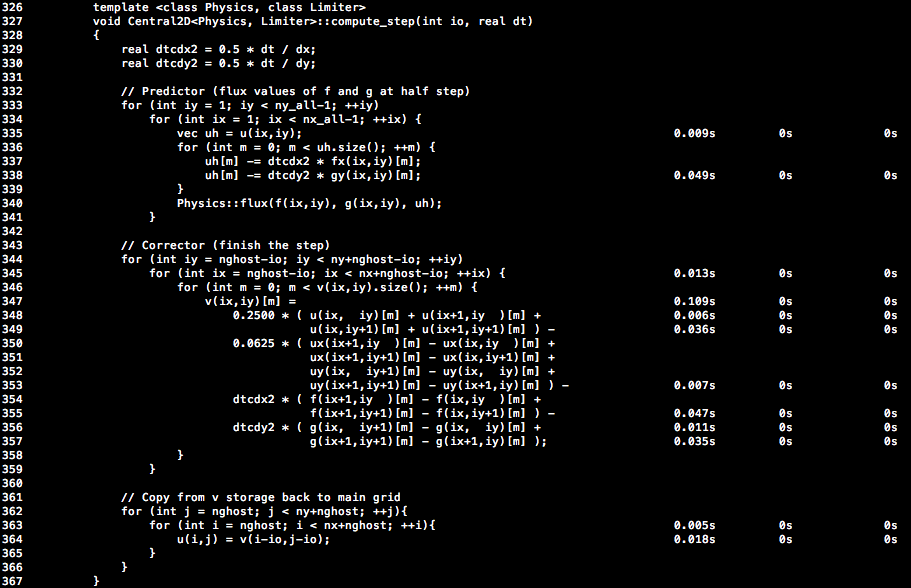
\includegraphics[width=0.8\linewidth]{vtune_origcode_computestep.png}
 % \caption{compute step function timings}
 % \label{fig2}
%\end{figure}


\section*{Serial Performance}

Include: initial profiling and vtune images (which was run for nx=800 and only threads=1 and timef = 1 for the original and final c versions)


\section*{Vectorization}
?

\section*{OpenMP Parallelization }
timef plots here? 

\section*{Domain Decomposition}
Can include scaling graphs here? For scaling, definitely want to include strong and weak scaling formulae and data. 

Not entirely sure why the scaling all works in given ways...

\section*{Processor Offloading}
Command: \#pragma offload target(mic:thread) to offload to xeon phis

Strong scaling is viewable in the strong scaling efficiency graph - better scaling than both original and new c codes on the compute nodes. However, timings for equivalent runs take longer.


\end{document}